\documentclass[preview]{standalone}
\usepackage{amsmath} 
\usepackage{amssymb} 
\usepackage{tikz}
\usepackage{array}
\begin{document}
\begin{tabular}[t]{m{6cm}m{9cm}}
  \vbox{\begin{align*}
    p_1 &: S_\alpha \rightarrow S_\beta \\
    p_2 &: S_\beta \rightarrow S_\gamma \\
    p_2 \circ p_1 &: S_\alpha \rightarrow S_\gamma \\
    (p_2 \circ p_1)&(s)\equiv p_2(p_1(s))
  \end{align*}}
  &
  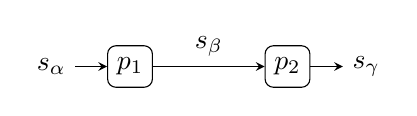
\begin{tikzpicture}[baseline={(sa.south)}, every node/.style={rounded corners=3pt}]
    \node[draw, minimum size=15pt] (p1) at (0,0) {$p_1$}; 
    \node[draw, minimum size=15pt] (p2) at (2,0) {$p_2$};
    \node[] (sa) at (-1,0) {$s_\alpha$}; 
    \node[anchor=south] (sb) at (1,0) {$s_\beta$}; 
    \node[] (sg) at (3,0) {$s_\gamma$};
    \draw[-stealth] (sa) -- (p1); \draw[-stealth] (p1) -- (p2);
    \draw[-stealth] (p2) -- (sg);
  \end{tikzpicture}
\end{tabular}

\end{document}

%%% Local Variables:
%%% mode: latex
%%% TeX-master: t
%%% End:
